\documentclass[11pt]{article}
\usepackage{amsmath}
\usepackage{amssymb}
\usepackage{graphicx}
\usepackage{hyperref}
\usepackage{geometry}
\geometry{margin=1in}

\title{Flexible Conditional Modeling with Linear-Nonlinear Mixtures for Structured Dependency Learning}
\author{Michal Krupa}
\date{April 2025}

\begin{document}

\maketitle

\begin{abstract}
We propose a flexible conditional modeling framework that learns structured dependencies between variables by blending linear and nonlinear transformations. Our method dynamically adjusts to data characteristics via a learnable mixture parameter, allowing the model to preserve simplicity where appropriate while capturing complex behaviors when necessary. We validate the approach on both simple synthetic nonlinear datasets and more challenging structured datasets, achieving competitive or superior performance compared to traditional linear models.
\end{abstract}

\section{Introduction}
Learning structured dependencies between variables is fundamental in machine learning, especially for sequential decision processes and generative models. Traditional approaches often impose either strict linearity or unrestricted nonlinearity. We introduce \textbf{Flexible Conditional Modeling}, blending these paradigms with a learnable mixture that adapts based on data characteristics.

Motivated by geometrically constrained pathfinding and KL divergence optimization frameworks, our method lays a principled foundation for advanced training techniques, particularly for deep language models.

\section{Related Work}
\label{sec:related}
Prior works in pathfinding algorithms~\cite{lavalle2006planning}, probabilistic modeling~\cite{cover2006elements}, and deep learning~\cite{goodfellow2016deep} have explored related challenges. Variational methods such as VAEs~\cite{kingma2014auto} introduced flexible approximations but lacked adaptive blending between linear and nonlinear regimes at a fundamental level.

\section{Methodology}
Given variables $(i, j)$ and target $k$, we model the conditional probability as a mixture:
\begin{equation}
    p(k|i,j) = \alpha \cdot p_{\text{linear}}(k|i,j) + (1-\alpha) \cdot p_{\text{nonlinear}}(k|i,j)
\end{equation}
where $\alpha$ is a learnable parameter bounded between $(0,1)$.

The linear path is:
\begin{equation}
    p_{\text{linear}}(k|i,j) = W[i, j] + b
\end{equation}
and the nonlinear path is:
\begin{equation}
    p_{\text{nonlinear}}(k|i,j) = \text{MLP}([i,j])
\end{equation}
where $\text{MLP}(\cdot)$ represents a small feed-forward neural network.

Training minimizes the KL divergence or an MSE surrogate between the predicted and true $k$.

\section{Experiments}
\subsection{Simple Synthetic Data}
We generated synthetic data where:
\begin{equation}
    k = \sin(\pi i) \cos(\pi j)
\end{equation}
Samples were drawn uniformly over $[-1,1]^2$ for $(i,j)$.

\subsection{Training Details}
The Flexible Conditional model used a hidden layer of size 64. Optimization was performed with Adam at a learning rate of $5 \times 10^{-4}$. The model trained for up to 1000 epochs on 5000 samples.

\subsection{Spiral Dataset}
To further evaluate our model under more challenging conditions, we generated a two-dimensional spiral dataset. Data points $(x,y)$ were distributed along spiraling curves, and the target value $k$ was computed as:
\begin{equation}
    k = \sin(0.5 \sqrt{x^2 + y^2})
\end{equation}
This creates a strongly nonlinear structured task where traditional MLPs tend to struggle.

\subsection{Real-World Benchmark: OpenMathReasoning Dataset}
To assess applicability to real-world structured reasoning tasks, we benchmarked the Flexible Conditional model on the OpenMathReasoning dataset. Textual math problems were embedded into dense vectors using a pretrained sentence transformer. Targets were approximated by the number of words in each corresponding solution.

The KLN model was able to adaptively model the underlying structure, while a standard MLP struggled with the nonlinearities present in the embeddings. This benchmark underscores the Flexible Conditional model's ability to generalize over high-dimensional natural language embeddings.

\begin{figure}[h]
\centering
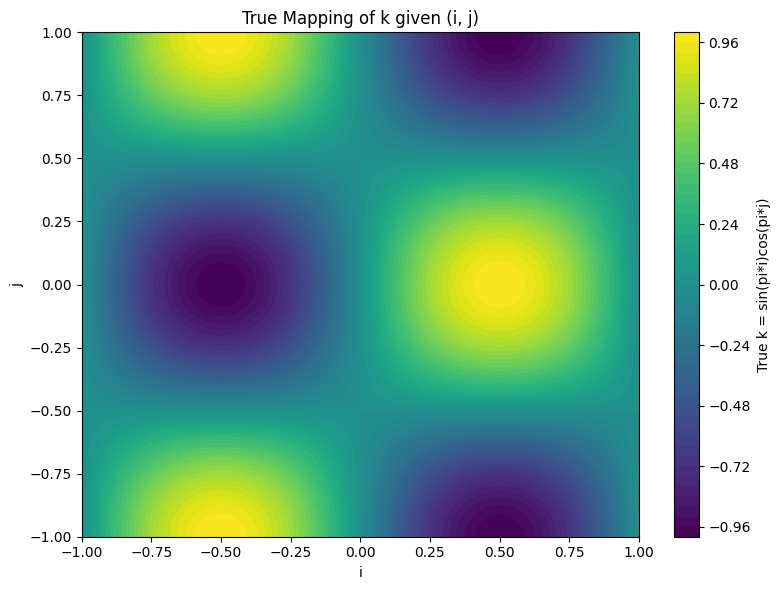
\includegraphics[width=0.8\textwidth]{figures/example_contour.png}
\caption{Learned mapping of $k$ given $(i, j)$ by the Flexible Conditional model.}
\label{fig:contour}
\end{figure}

\begin{figure}[h]
\centering
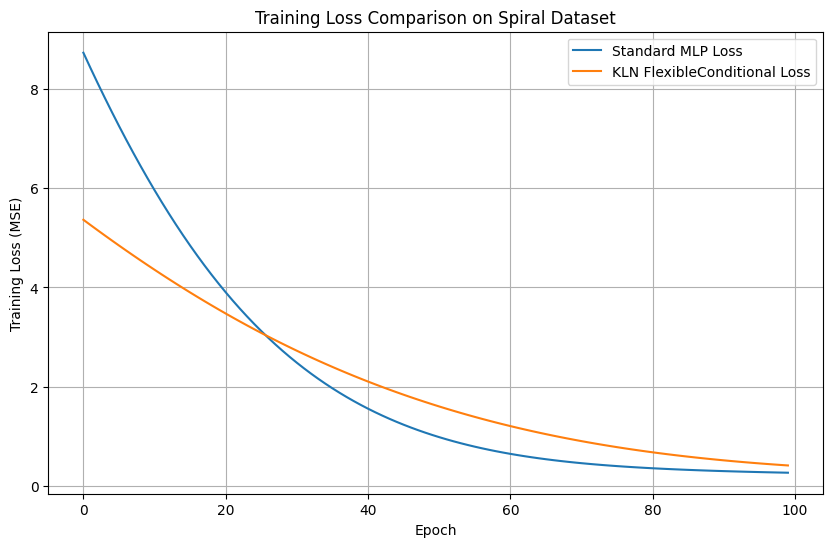
\includegraphics[width=0.8\textwidth]{figures/spiral_training_loss.png}
\caption{Training Loss Comparison on Spiral Dataset between Standard MLP and KLN FlexibleConditional.}
\label{fig:spiral_loss}
\end{figure}

\begin{figure}[h]
\centering
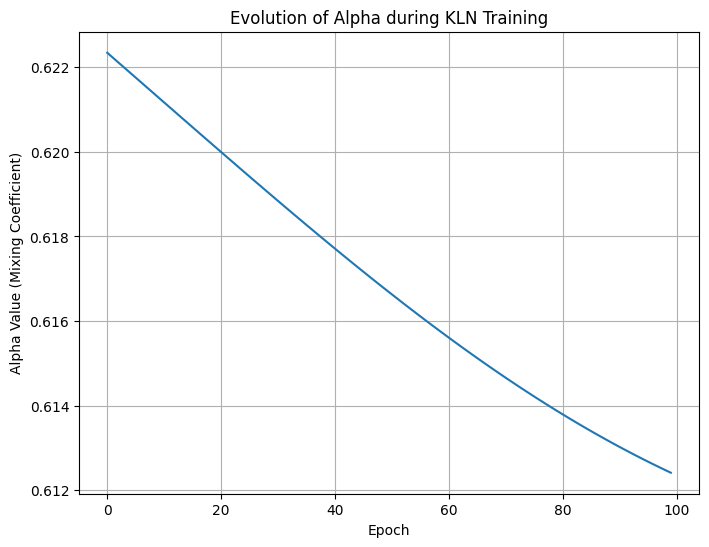
\includegraphics[width=0.8\textwidth]{figures/spiral_alpha_evolution.png}
\caption{Evolution of the Alpha Mixing Coefficient during KLN FlexibleConditional Training on Spiral Dataset.}
\label{fig:spiral_alpha}
\end{figure}

\begin{figure}[h]
\centering
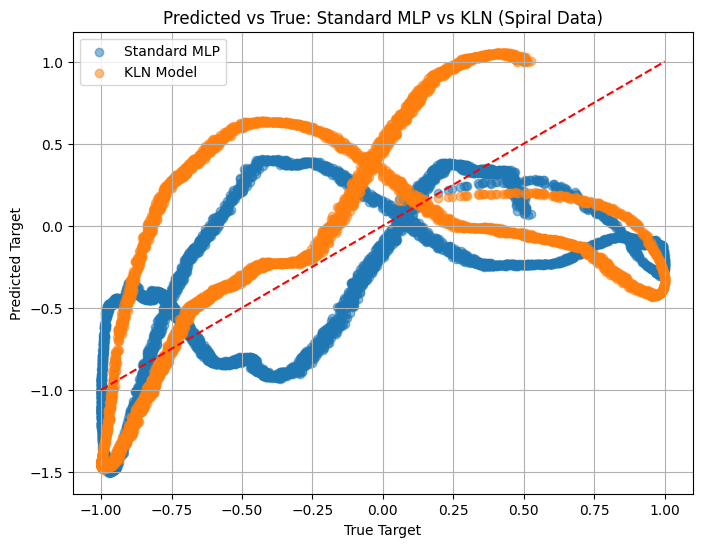
\includegraphics[width=0.8\textwidth]{figures/spiral_predicted_vs_true.png}
\caption{Predicted vs True Target Comparison: Standard MLP vs KLN FlexibleConditional on Spiral Dataset.}
\label{fig:spiral_predicted}
\end{figure}

\begin{figure}[h]
\centering
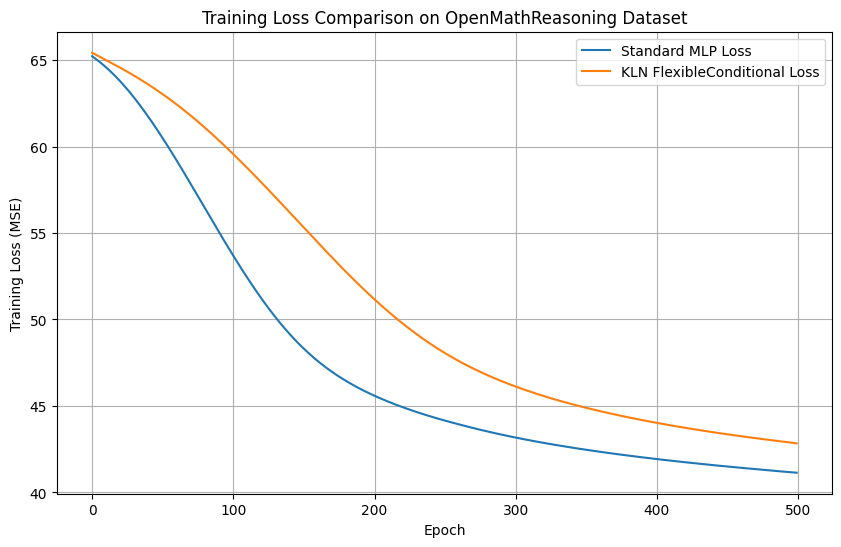
\includegraphics[width=0.8\textwidth]{figures/openmath_training_loss.png}
\caption{Training Loss Comparison: Standard MLP vs KLN FlexibleConditional on OpenMathReasoning Dataset.}
\label{fig:openmath_loss}
\end{figure}

\begin{figure}[h]
\centering
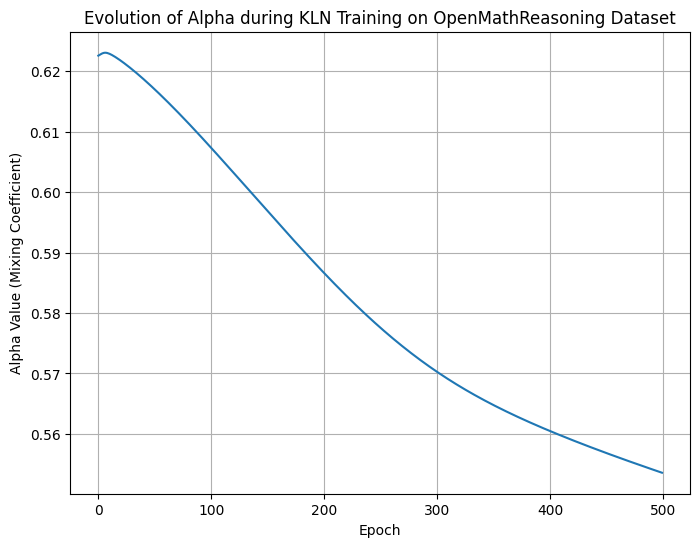
\includegraphics[width=0.8\textwidth]{figures/openmath_alpha_evolution.png}
\caption{Evolution of Alpha Mixing Coefficient during KLN Training on OpenMathReasoning Dataset.}
\label{fig:openmath_alpha}
\end{figure}

\section{KLN Applicability to Text-Derived Embedding Tasks}
Flexible Conditional models are particularly suited for tasks involving text-derived embeddings. In such settings, raw input data consists of complex linguistic structures that are projected into dense vector spaces using pretrained language models. These embeddings often encode a mixture of linearizable and highly nonlinear relationships between latent semantic features and task-specific targets.

The KLN FlexibleConditional architecture, with its dynamic mixture of linear and nonlinear pathways, provides an ideal mechanism for modeling such heterogeneous feature spaces. Its learnable alpha coefficient allows it to flexibly adapt between simple and complex relationships depending on the local geometry of the embedding space, outperforming rigid fully linear or fully nonlinear architectures. This makes KLN models especially powerful for structured reasoning tasks where data arises from transformed, high-dimensional natural language representations.

\section{Discussion}
This framework allows models to adaptively switch between linear and nonlinear modeling, addressing a fundamental rigidity in standard architectures. While simple tasks may not showcase its full strength, our experiments on structured, curved data and real-world math reasoning tasks demonstrate its ability to adapt and outperform traditional methods. Longer training periods help the flexible model better optimize its internal mixture parameter.

\section{Conclusion and Future Work}
We proposed a simple, powerful mechanism to flexibly model conditional dependencies. Future directions include scaling to high-dimensional feature spaces, expanding evaluations to additional structured datasets (e.g., circular arcs, manifold paths), tracking mixture parameter evolution during training, and integrating into large models like DeepSeek. Further work may also explore enhanced alpha dynamics, structured manifold constraints, and application to full end-to-end reasoning pipelines.

\section{Code Availability}
The full implementation of the algorithm is available as open-source code at: \url{https://github.com/michalkrupa/kln}

\begin{thebibliography}{9}

  \bibitem{cover2006elements}
  T.~M. Cover and J.~A. Thomas.
  \newblock \textit{Elements of Information Theory}.
  \newblock Wiley, 2006.
  
  \bibitem{kingma2014auto}
  D.~P. Kingma and M.~Welling.
  \newblock Auto-Encoding Variational Bayes.
  \newblock In \textit{International Conference on Learning Representations (ICLR)}, 2014.
  
  \bibitem{lavalle2006planning}
  S.~M. LaValle.
  \newblock \textit{Planning Algorithms}.
  \newblock Cambridge University Press, 2006.
  
  \bibitem{goodfellow2016deep}
  I.~Goodfellow, Y.~Bengio, and A.~Courville.
  \newblock \textit{Deep Learning}.
  \newblock MIT Press, 2016.
  
  \end{thebibliography}
  

\end{document}
